% !TeX root = paper.tex
\section{Elementary Perceptual Tasks}

Cleveland and McGill describe the mapping of graphical elements to quantitative variables as \emph{elementary perceptual tasks} and introduce a list of ten different encodings in their paper~\cite{cleveland_mcgill}. These tasks are the low-level building blocks for information visualizations and encode quantities. Cleveland and McGill did not explicitly test human perception of single instances of these encodings. However, we test how each classifier measures encoded values using the elementary perceptual tasks and create visualizations of these tasks as rasterized images with different parametrizations (Table~\ref{tab:encoding_parameters}).

\subsection{Parametrizations}
\label{sec:parametrizations}
We generate multiple parameterizations for each elementary perceptual task and sequentially increase the number of parameters (Table~\ref{tab:encoding_parameters}). For instance, for \emph{Position Common Scale} we first only vary the $y$-position which yields just $60$ different parameters. We then include translation along the x-axis with a significant increase in variability. We then also add a variable spot size. This results in more complex datasets depending on the increase of variability. Table~\ref{tab:encoding_parameters} shows the different settings. It is important to consider this variability when evaluating different classifiers with individual trainable parameters (Table~\ref{tab:parameters}). In theory, classifiers can memorize the images if the data set has a low variability. We also counteract such behavior by adding noise.

%\begin{figure}[t]
%	  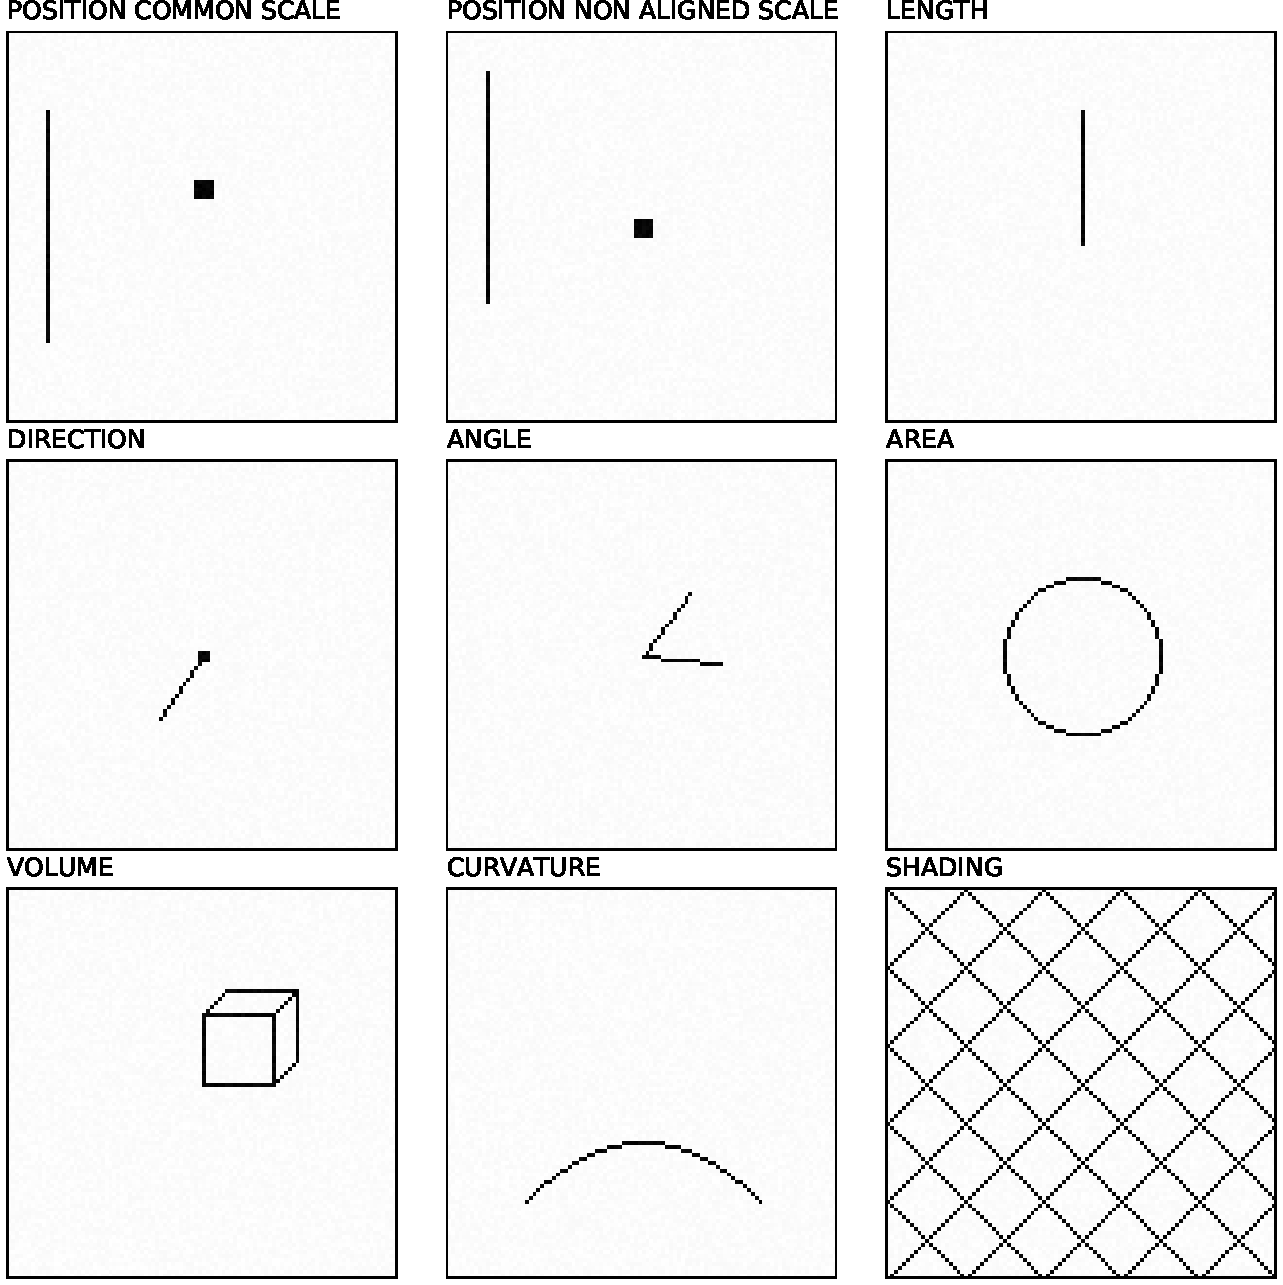
\includegraphics[width=\linewidth]{figure1_overview.pdf}
%  \caption{\textbf{Elementary Perceptual Tasks.} Rasterized visualizations of the elementary perceptual tasks as defined by Cleveland and McGill~\cite{cleveland_mcgill} (color saturation excluded). We vary the parameters of each perceptual task and then assess the interpretability of feed-forward neural networks.}
%	\label{fig:elementary_perceptual_tasks}
%\end{figure}
\begin{table}[h]
\centering
\caption{\textbf{Elementary Perceptual Tasks.} Rasterized visualizations of the elementary perceptual tasks as defined by Cleveland and McGill~\cite{cleveland_mcgill} (color saturation excluded). We sequentially increase the number of parameters (e.g. by adding translation) for every task. This introduces variability and creates increasingly more complex datasets.}
\resizebox{\linewidth}{!}{
\begin{tabular}{lllr}
	\toprule
	\multicolumn{2}{l}{Elementary Perceptual Task} & ~ & Permutations\\
	\midrule
	\raisebox{-.85\height}{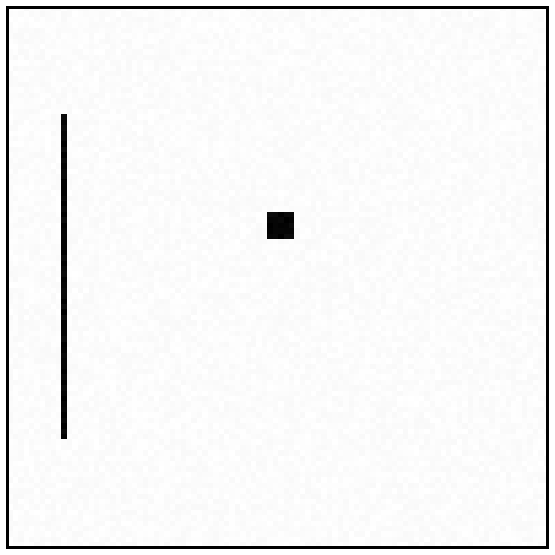
\includegraphics[width=.5in]{position_common_scale.pdf}} & \makecell[tl]{\emph{Position Common Scale}\\~~~Position Y\\~~~+ Position X \\~~~+ Spot Size \\} &~& \makecell[tr]{~\\ $60$ \\ $3,600$ \\ $216,00$}\\

	\midrule
	\raisebox{-.85\height}{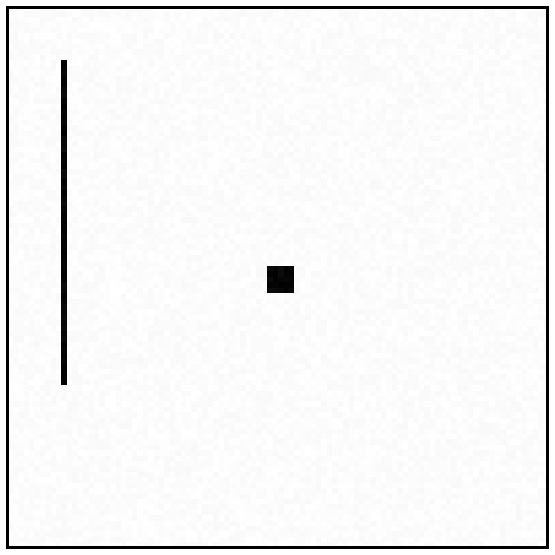
\includegraphics[width=.5in]{position_non_aligned_scale.pdf}} & \makecell[tl]{\emph{Position Non-Aligned Scale}\\~~~Position Y\\~~~+ Position X \\~~~+ Spot Size \\} &~& \makecell[tr]{~\\ $600$ \\ $36,000$ \\ $216,000$}\\

	\midrule
	\raisebox{-.95\height}{
\includegraphics[width=.5in]{length.pdf}} & \makecell[tl]{\emph{Length}\\~~~Length\\~~~+ Position Y \\~~~+ Position X \\~~~+ Width} &~& \makecell[tr]{ ~\\$60$ \\ $2,400$ \\ $144,000$\\$864,000$}\\

	\midrule
	\raisebox{-.85\height}{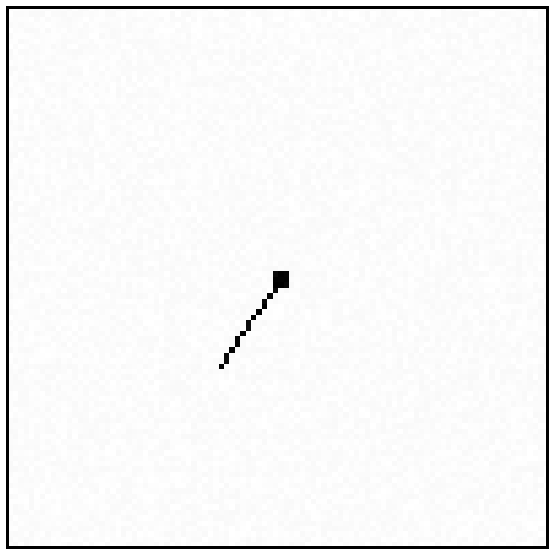
\includegraphics[width=.5in]{direction.pdf}} & \makecell[tl]{\emph{Direction}\\~~~Angle\\~~~+ Position Y \\~~~+ Position X} &~& \makecell[tr]{ ~\\$360$ \\ $21,600$ \\ $1,296,000$}\\

	\midrule
	\raisebox{-.85\height}{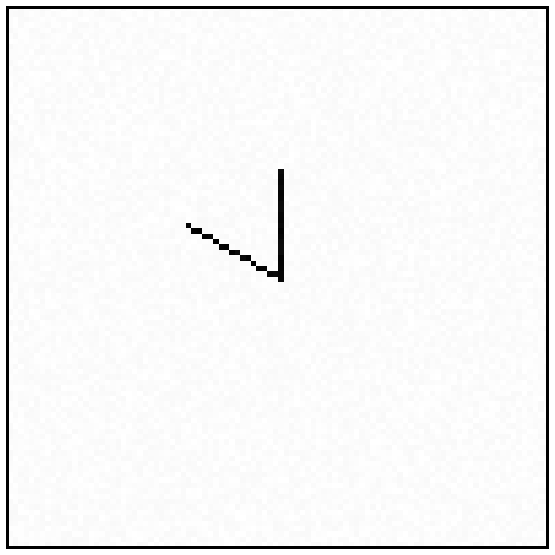
\includegraphics[width=.5in]{angle.pdf}} & \makecell[tl]{\emph{Angle}\\~~~Angle\\~~~+ Position Y \\~~~+ Position X} &~& \makecell[tr]{ ~\\$90$ \\ $5,400$ \\ $324,000$}\\

	\midrule
	\raisebox{-.85\height}{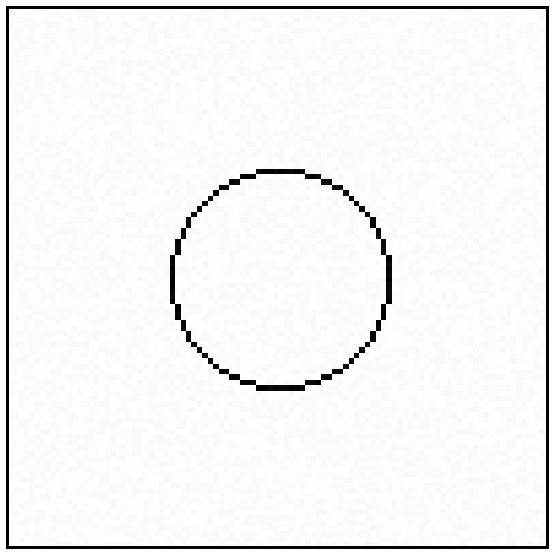
\includegraphics[width=.5in]{area.pdf}} & \makecell[tl]{\emph{Area}\\~~~Radius\\~~~+ Position Y \\~~~+ Position X} &~& \makecell[tr]{ ~\\$40$ \\ $800$ \\ $16,000$}\\

	\midrule
	\raisebox{-.85\height}{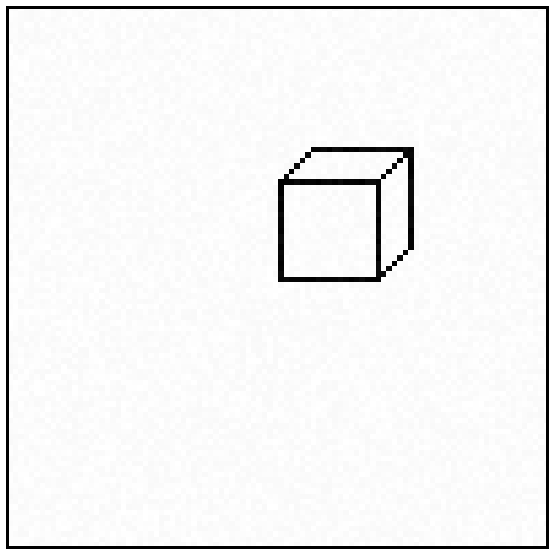
\includegraphics[width=.5in]{volume.pdf}} & \makecell[tl]{\emph{Volume}\\~~~Cube Sidelength\\~~~+ Position Y \\~~~+ Position X} &~& \makecell[tr]{ ~\\$20$ \\ $400$ \\ $8,000$}\\
	
	\midrule
	\raisebox{-.85\height}{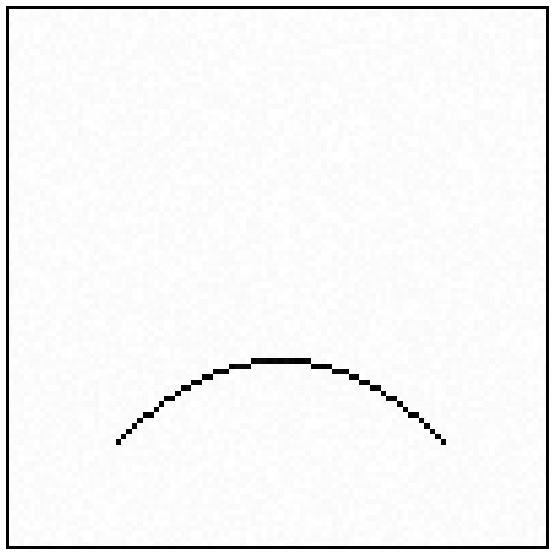
\includegraphics[width=.5in]{curvature.pdf}} & \makecell[tl]{\emph{Curvature}\\~~~Midpoint Curvature\\~~~+ Position Y \\~~~+ Position X} &~& \makecell[tr]{ ~\\$80$ \\ $1,600$ \\ $64,000$}\\	

	\midrule
	\raisebox{-.85\height}{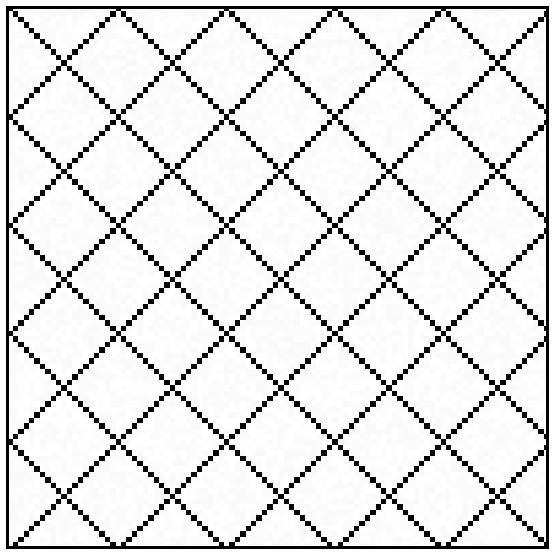
\includegraphics[width=.5in]{shading.pdf}} & \makecell[tl]{\emph{Shading}\\~~~Density\\~~~+ Position Y \\~~~+ Position X} &~& \makecell[tr]{ ~\\$100$ \\ $2,000$ \\ $40,000$}\\	
%	
	\bottomrule
\end{tabular}
}
\label{tab:encoding_parameters}
\end{table}

\subsection{Hypotheses}

We proposed four hypotheses entering the elementary perceptual task experiment:

\begin{itemize}
	\item \textbf{H1.1} \textbf{Visual cortex inspired classifiers are able to connect graphical elements to their quantitative variables.} While much simpler models than their biological pendant, convolutional neural networks are heavily influenced by our biological knowledge of the visual system. Such classifiers therefor follow the same principles as human perception.
	\item \textbf{H1.2} \textbf{Computed perceptual performance is dependent on classifier complexity.} We evaluate multiple classifiers with different numbers of trainable parameters. A more complex classifier (with higher number of parameters) will perform better on elementary perceptual tasks.
	\item \textbf{H1.3} \textbf{Some visual encodings are better than others for computations.} Cleveland and McGill order the elementary perceptual tasks by accuracy. We investigate whether this order is also relevant for computing graphical perception.
	\item \textbf{H1.4} \textbf{Classifiers trained on perceptual tasks can generalize to more or less complex variations of the same task.} Recent research suggests that convolutional neural networks generalize extremely well. While the underlying reasons are mainly yet unknown, this property allows them to perform on variations of a similar perceptual task.
\end{itemize}

\subsection{Results}


some are good and some are bad.. why?

\begin{figure*}[h]
	\centering
	  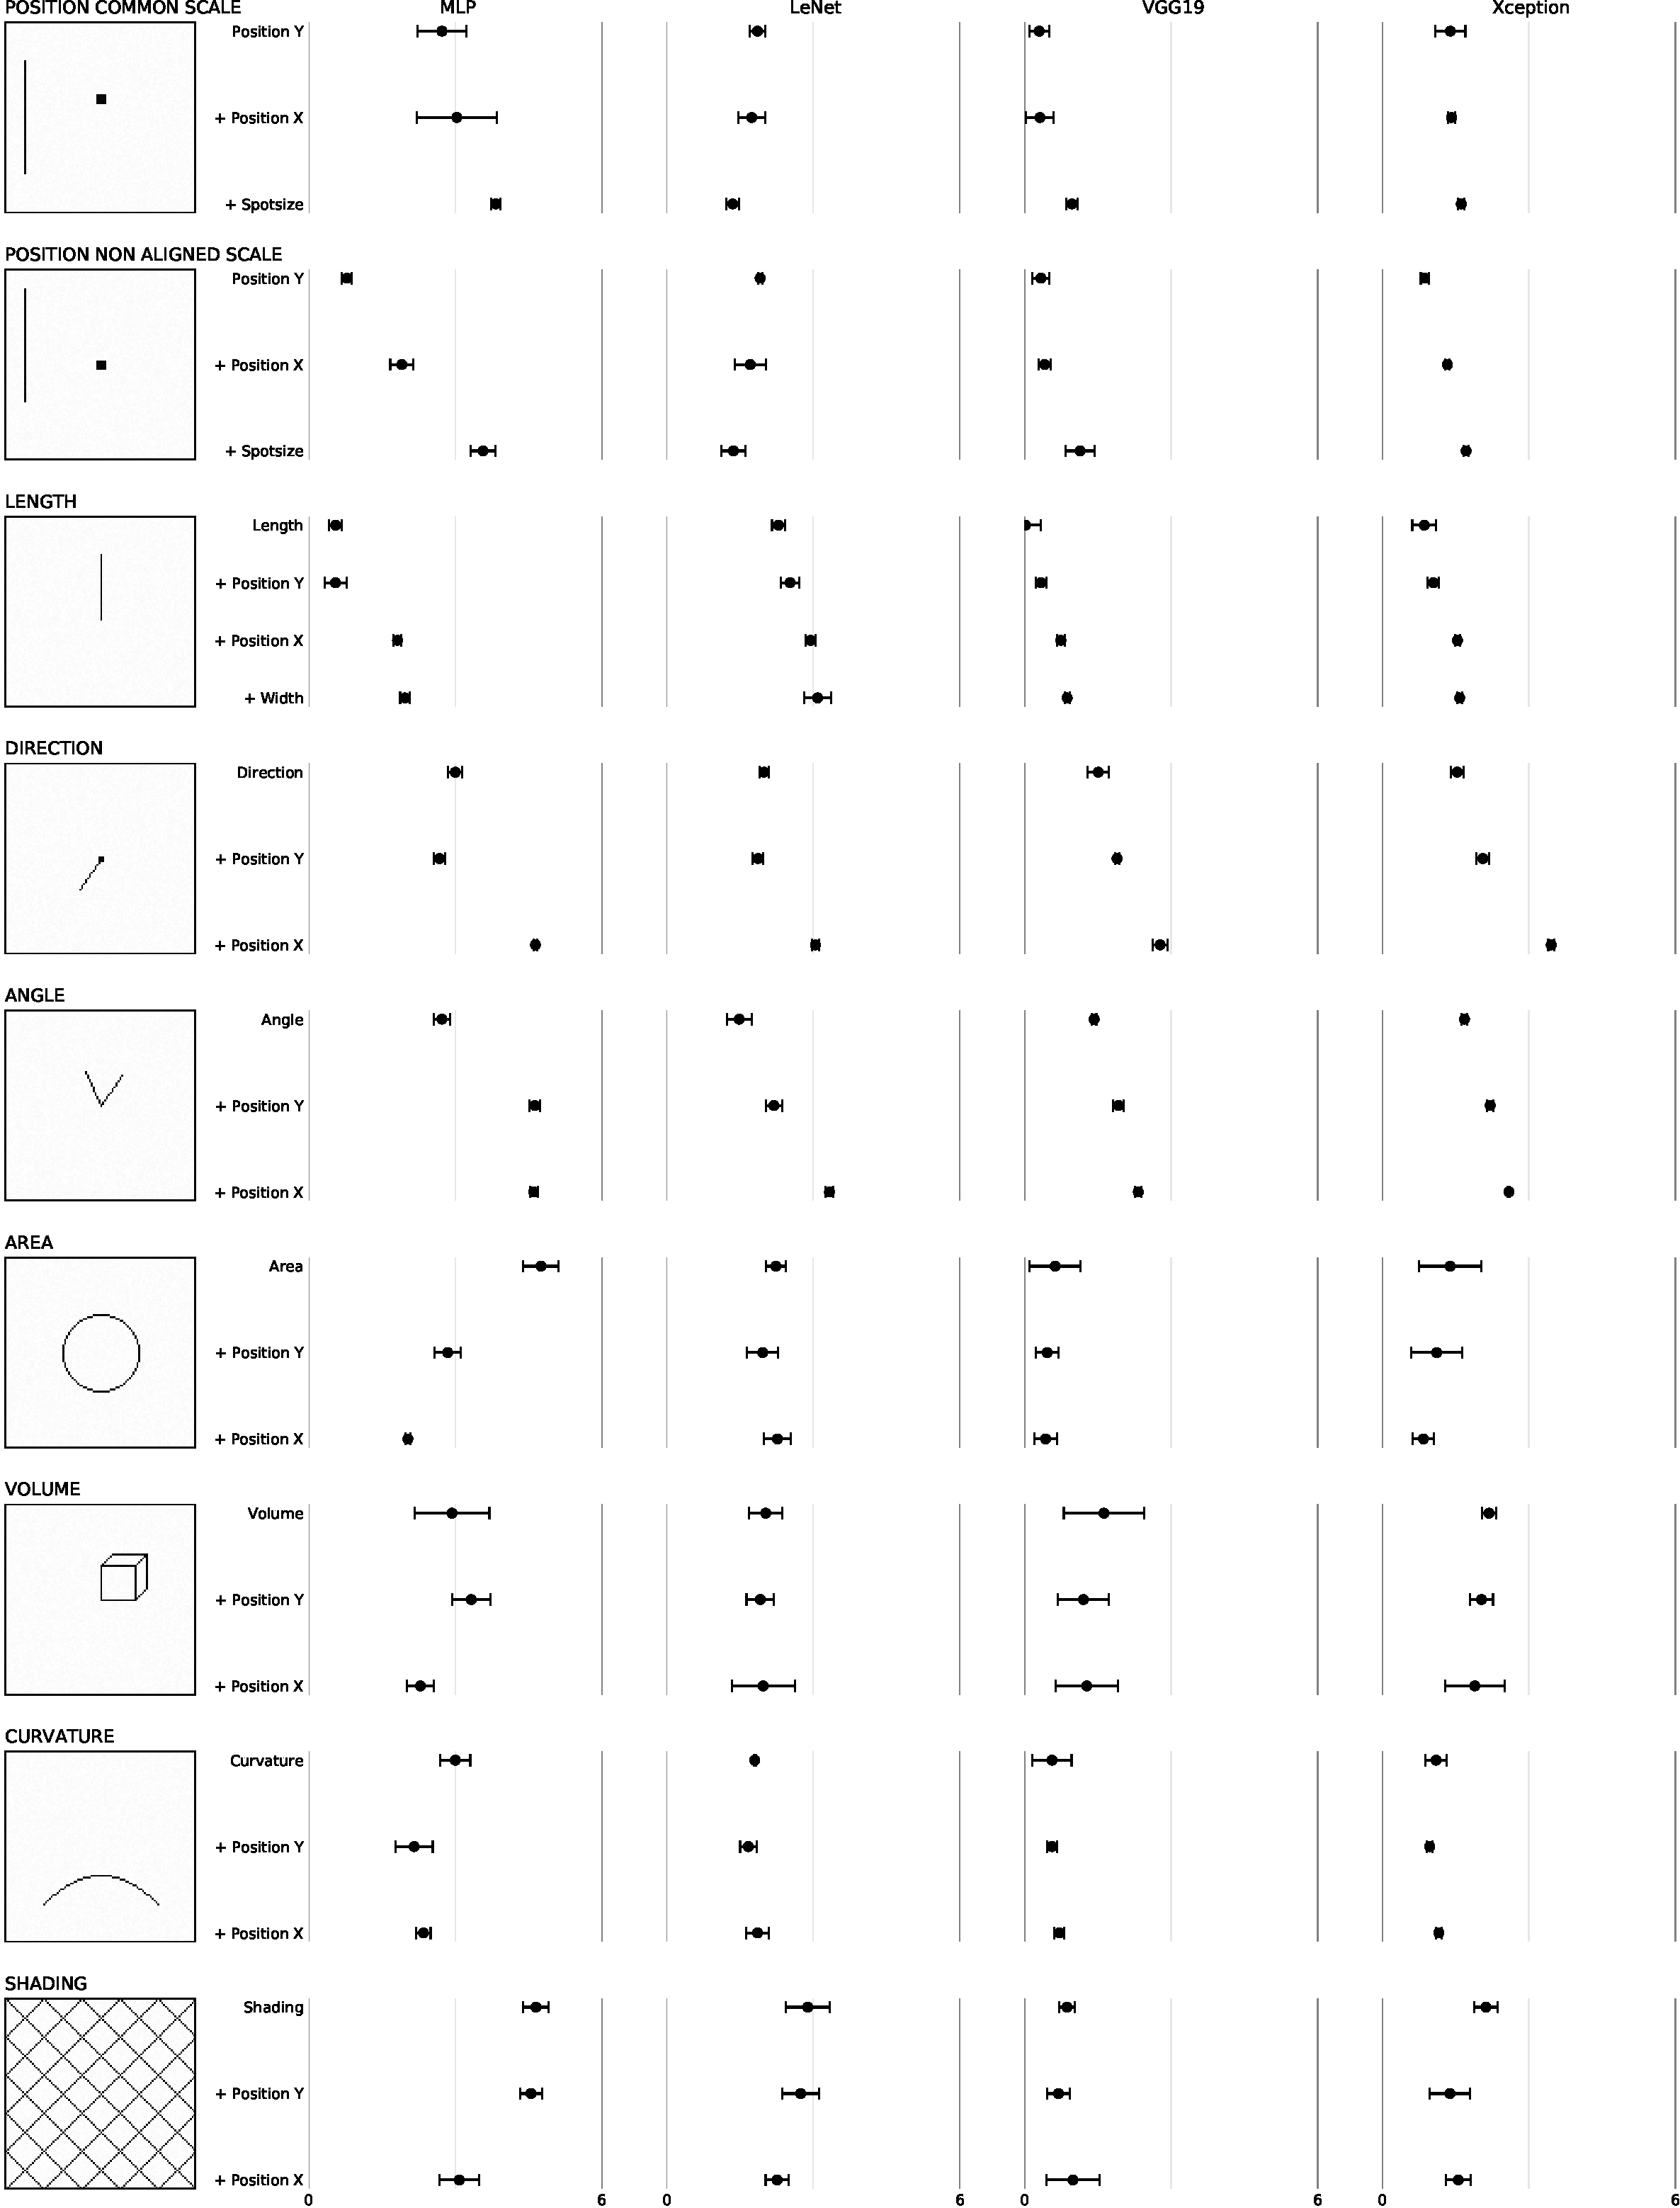
\includegraphics[width=.95\linewidth]{figure1.pdf}
  \caption{\textbf{Computational results of Elementary Perceptual Tasks experiment.} Log absolute error means and 95\% confidence intervals for computed perception of different classifiers on the \emph{elementary perceptual tasks} introduced by Cleveland and McGill 1984~\cite{cleveland_mcgill}. We test the performance of a Multi-layer Perceptron (MLP), the LeNet Convolutional Neural Network, as well as feature generation using the VGG19 and Xception networks trained on ImageNet.}
	\label{fig:figure1_results}
\end{figure*}

\textbf{Computational Perception Ranking.}

Cleveland McGills Ranking - can we observe something similar?

\begin{enumerate}
	\item Position along a common scale e.g. scatter plot
	\item Position on identical but nonaligned scales e.g. multiple scatter plots
	\item Length e.g. bar chart
	\item Angle \& Slope (tie) e.g. pie chart
	\item Area e.g. bubbles
	\item Volume, density, and color saturation (tie) e.g. heatmap
	\item Color hue e.g. newsmap
\end{enumerate}

\noindent{\textbf{Cross-classifier variability.}}

Can a neural network generalize on simple perceptual tasks?

\begin{figure}[t]
	  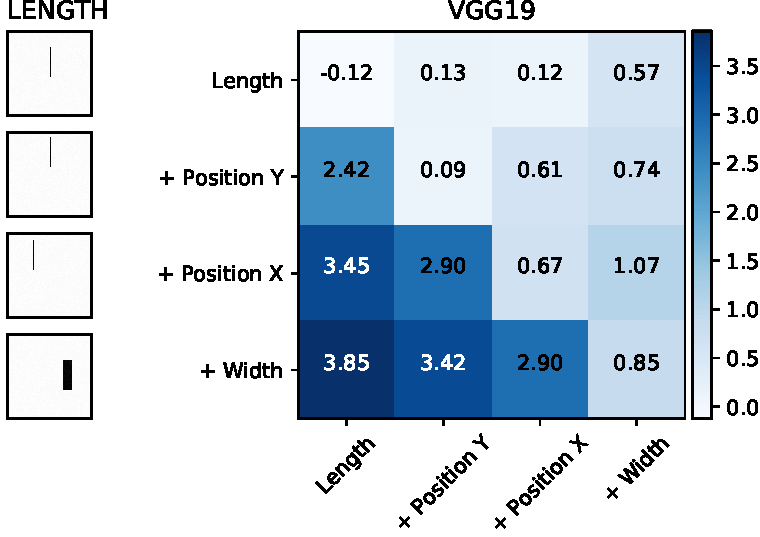
\includegraphics[width=\linewidth]{cross_network_small_VGG19.pdf}
  \caption{\textbf{Cross-classifier variability for the perceptual task of measuring length.} We use predictions of LeNet classifiers trained on different parametrizations of the \emph{curvature} elementary perceptual task and measure the mean logistic absolute error (MLAE). The lower score, the better. Classifiers trained on curves with variable position can generalize even if the axis of translation varies. However, classifiers trained on fixed positions of curves are not able to measure translated curves.}
	\label{fig:cross_network}
\end{figure}
